% shared/template.tex
%
% Contiene un modello di documento che deve essere copiato e opportunamente
% modificato per creare i documenti 'concreti' di progetto. Definisce le macro
% specifiche per il documento corrente, importa la parte di preambolo condivisa
% e le pagine comuni a tutti i documenti.
% In particolare, per ogni documento concreto occorre per prima cosa aggiornare
% le macro, inserire una voce nella tabella delle modifiche e inserire il testo
% (o includere file sorgenti esterni) a partire dalla riga 66 in poi.

% **************************************************
% Macro specifiche per il documento corrente
% **************************************************
% Nome
\newcommand{\docName}{Norme di Progetto}
% Nome file
\newcommand{\docFileName}{norme\_di\_progetto.1.0.pdf}
% Versione
\newcommand{\docVers}{1.0}
% Data creazione
\newcommand{\creationDate}{2012-12-01}
% Data ultima modifica
\newcommand{\modificationDate}{2012-12-04}
% Stato in {Approvato, Non approvato}
\newcommand{\docState}{Approvato}
% Uso in {Interno, Esterno}
\newcommand{\docUsage}{Interno}
% Redattori da specificare come nome1\\ &nome2\\ ecc.
\newcommand{\docAuthors}{Andrea Meneghinello}
% Approvato da
\newcommand{\approvedBy}{Stefano Farronato}
% Verificatori
\newcommand{\verifiedBy}{Marco Schivo}
% Perscorso (relativo o assoluto) che punta alla directory contenente shared/
% come sua sottodirectory (per comodità chiamiamola 'doc root').
\newcommand{\docRoot}{..}
% definire se si vuole l'indice delle tabelle
\def\INDICETABELLE{true}
% definire se si vuole l'indice delle figure
\def\INDICEFIGURE{true}

% importa il preambolo condiviso da tutti i documenti
% shared/preamble.tex
%
% Questo documento contiene la parte del preambolo condivisa e viene pertanto
% richiamato nel 'master' di tutti i documenti di progetto.  Al suo interno
% contiene le inclusioni (e le configurazioni) di tutti i package richiesti per
% la compilazione dei documenti, le macro di carattere generale e la definizione
% degli stili di pagina.

\documentclass[a4paper,10pt,openright]{article}

% **************************************************
% Macro generiche
% **************************************************
\newcommand{\team}{Software Synthesis}                    % chi siamo
\newcommand{\email}{software.synthesis@gmail.com}         % e-mail
\newcommand{\caName}{}                                    % titolo capitolato
\newcommand{\caDescr}{}                                   % descrizione
\newcommand{\inglese}[1]{\textit{#1}}

% **************************************************
% Codifica e lingua dei documenti
% **************************************************
\usepackage[utf8x]{inputenc}                              % codifica caratteri dei documenti sorgenti
\usepackage[english,italian]{babel}                       % localizzazione ai fini di sillabazione e cross-references
\usepackage[T1]{fontenc}                                  % codifica font di output

% **************************************************
% Definizione geometria della pagina
% **************************************************
\usepackage[a4paper,head=4cm,top=4.5cm,bottom=3cm,left=3cm,right=3cm,bindingoffset=5mm]{geometry}

% *************************************************
% Intestazioni e piè di pagina personalizzati
% *************************************************
\usepackage{fancyhdr}
% stile normale
\fancypagestyle{normal}{
\fancyhead{}                                              % intestazione
\fancyhead[RE,RO]{
\begin{picture}(0,0)
  \put(-410,0){
\includegraphics[width=1.02\textwidth]{header_logo}}
  \put(-410,10){\sffamily\large\leftmark}
\end{picture}
\vspace{-4pt}
}
\renewcommand{\headrulewidth}{.4pt}                       % riga sotto l'intestazione
\cfoot{}                                                  % piè di pagina
\fancyfoot[RO,LE]{\sffamily
  pag.~\thepage{} di \pageref{LastPage}}                  % a dx nelle pag. dispari e a sx in quelle pari
\fancyfoot[RE,LO]{\sffamily\docFileName{} -- v.\docVers}
\renewcommand{\footrulewidth}{.4pt}                       % riga sopra il piè di pagina
}
% stile per gli indici
\fancypagestyle{toc}{
\fancyhead{}                                              % intestazione
\fancyhead[RE,RO]{
\begin{picture}(0,0)
  \put(-410,0){
\includegraphics[width=1.02\textwidth]{header_logo}}
\end{picture}
}
\renewcommand{\headrule}{}                                % nessuna riga sotto l'intestazione
\cfoot{}                                                  % piè di pagina
\fancyfoot[RO,LE]{\sffamily\thepage{}}                    % a dx nelle pag. dispari e a sx in quelle pari
\fancyfoot[RE,LO]{\sffamily\docFileName{} -- v.\docVers}
\renewcommand{\footrulewidth}{.4pt}                       % riga sopra il piè di pagina
}

\pagestyle{fancy}                                         % premetto: non so usare bene le marche:
\renewcommand{\sectionmark}[1]{\markboth{#1}{#1}}         % se qualcuno ha idee migliori si faccia avanti!

% **************************************************
% Tabelle
% **************************************************
\usepackage{tabularx}                                     % tabelle di larghezza fissa con una o più colonne variabili
\usepackage{multirow}                                     % colonne con colonne che si estendono per più righe
\usepackage{booktabs}                                     % per inserire l'ambiente table e le righe orizz. nelle tabelle
\usepackage{longtable}			                          % tabelle oltre i limiti di pagina

% **************************************************
% Cross-references e collegamenti ipertestuali
% **************************************************
\usepackage[hidelinks]{hyperref}
\hypersetup{%
  colorlinks=false, linktocpage=false, pdfborder={0,0,0}, pdfstartpage=3, pdfstartview=FitV,%
  urlcolor=Cyan, linkcolor=Cyan, citecolor=Black, %pagecolor=Black,%
  pdftitle={\docName}, pdfauthor={\team}, pdfsubject={}, pdfkeywords={},%
  pdfcreator={pdflatex}, pdfproducer={pdflatex with hyperref package}%
}

% **************************************************
% Immagini e grafica
% **************************************************
\usepackage{graphicx}                                     % supporto ad aspetti avanzati delle immagini
\graphicspath{{\docRoot/pics/}}                           % percorso contenente tutti i file immagini
\usepackage{color}                                        % permette di colorare facilmente il testo

% **************************************************
% Altri pacchetti opzionali
% **************************************************     
\usepackage{lastpage}                                     % per sapere il numero totale di pagine
\usepackage{lipsum}                                       % genera "dummy text" per prove di impaginazione
\usepackage{eurosym}                                      % per il simbolo dell'euro usare \EUR{x} dove x è l'importo


% Fine del preambolo e inizio del documento
\begin{document}

% Inclusione della prima pagina
% shared/firstpage.tex
%
% Questo documento definisce il contenuto della prima pagina, che si suppone
% essere uguale in tutti i documenti.  Oltre al logo e al titolo, la prima
% pagina contiene i metadati relativi al documento in cui viene inclusa.


% rimuove intestazioni e piè di pagina
\pagestyle{empty}

\begin{center}

% logo del gruppo

\includegraphics[width=1.5\textwidth]{logo}

\vspace{1in}

% titolo del documento
{\Huge\bfseries \docName}

\vspace{1in}

% tabella riepilogativa
\begin{tabularx}{.7\textwidth}{>{\bfseries\sffamily}l>{\sffamily}l}
\toprule
\multicolumn{2}{>{\sffamily}c}{Informazioni sul documento}\\
\midrule
Nome file:            & \docFileName\\
Versione:             & \docVers\\
Data creazione:       & \creationDate\\
Data ultima modifica: & \modificationDate\\
Stato:                & \docState\\
Uso:                  & \docUsage\\
Redattori:            & \docAuthors\\
Approvato da:         & \approvedBy\\
Verificatori:         & \verifiedBy\\
\bottomrule
\end{tabularx}

\end{center}

\newpage


% Storico delle modifiche
\section*{Storia delle modifiche}
\begin{tabularx}{\textwidth}{lXll}
\toprule
Versione & Descrizione intervento & Redattore & Data\\
\midrule % inserire qui il contenuto della tabella
1.0 & Approvazione documento & Stefano Farronato & 2012-12-04\\
0.6 & Validazione documento & Marco Schivo & 2012-12-04\\
0.5 & Fine stesura documento & Andrea Meneghinello & 2012-12-03\\
0.4 & Stesura sezione Milestones e Ticketing, Analisi dei requisiti & Andrea Meneghinello & 2012-12-03\\
0.3 & Stesura sezione ambiente documentale & Andrea Meneghinello & 2012-12-03\\
0.2 & Stesura sezione ambiente di lavoro & Andrea Meneghinello & 2012-12-01\\
0.1 & Stesura scheletro documento, sezione comunicazione & Andrea Meneghinello & 2012-12-01\\
\bottomrule
\end{tabularx}
\newpage

% inclusione dell'indice
% shared/toc.tex
%
% Questo file contiene le istruzioni che generano l'indice o gli indici del
% documento (utile nel caso in cui decidessimo di avere anche un indice delle
% tabelle e/o un indice delle figure).

\pagestyle{toc}
\pagenumbering{roman}

\tableofcontents

\newpage


% Alcuni aggiustamenti per le pagine
\pagenumbering{arabic}
\setcounter{page}{1}
\pagestyle{normal}

\newpage
\section{Introduzione}
\subsection{Scopo del prodotto}
Con progetto ``MyTalk'' intendiamo un sistema software di comunicazione tra utenti mediante \underline{browser}, utilizzando solo componenti standard, senza dover installare \underline{plugin} o programmi esterni. L'utilizzatore dovrà poter chiamare un altro utente, iniziare la comunicazione sia audio che video, svolgere la chiamata e terminare la chiamata ottenendo delle statistiche sull'attività.

\subsection{Scopo del documento}
Questo documento viene redatto per definire le norme da adottare da parte di tutti i componenti del gruppo Software Synthesis durante il periodo di svolgimento del capitolato ``MyTalk'', commissionato dall'azienda Zucchetti SPA. In particolare si andranno a definire le regole per:
\begin{itemize}
\item Relazioni interpersonali e comunicazione
\item Definizione dell'ambiente di lavoro
\item Redazione documenti
\item Convenzioni e norme per l'analisi e la progettazione
\item Convenzioni e norme per la verifica di file e documenti
\end{itemize}

\subsection{Ambiguità}
Al fine di evitare incomprensioni dovute all'uso di termini tecnici nei documenti, viene redatto e allegato il documento ``Glossario.pdf'' dove vengono definiti e descritti tutti i termini marcati con una sottolineatura.

\newpage
\section{Relazioni interpersonali e comunicazione}
\subsection{Comunicazione interna}
\label{sec:comunicazione_interna}
La comunicazione tra i vari componenti del team avverrà principalmente durante gli incontri che si terranno in un luogo fisico comune. Per evitare problemi dovuti alla mancata presenza da parte di un membro, le notifiche dell'attività svolta durante l'incontro verranno scritte in un calendario comune messo a disposizione.
Nei casi in cui il lavoro si svolgerà presso la propria abitazione, si potrà utilizzare \textit{Skype} per avviare chat, chiamate e videoconferenze di gruppo.
Qualora si evinca la necessità di un ritrovo fisico comune ma vi è l'impossibilità da parte di alcuni membri di recarsi nel luogo prefissato, allora si procederà suddividendo il gruppo in due sottogruppi, ciascuno con un luogo di ritrovo prefissato. I due team di sviluppo quindi potranno comunicare con l'altro team mediante software di comunicazione prestabilito.


\subsection{Comunicazione esterna}
I contatti verso l'esterno saranno a cura del responsabile di progetto. A tale scopo è stato creato un indirizzo di posta elettronica tramite il quale la persona incaricata tratterà a nome dell'intero gruppo Software Synthesis. L'email sopra descritta è \textit{info@softwaresynthesis.org} e l'inoltro di risposte a tutti gli altri membri sarà sempre a carico del responsabile di progetto che dovrà utilizzare i metodi descritti nella sezione \ref{sec:comunicazione_interna} ``Comunicazione Interna''.

\subsection{Incontri Interni}
Saranno fissate delle riunioni formali decise dal responsabile di progetto che provvederà rendere noto a tutti luogo, data e ora della seduta mediante email personale con almeno tre giorni di anticipo. Nell'email sarà contenuta anche la motivazione per cui si è reso necessario l'incontro. Ai membri è richiesta la conferma di partecipazione tramite risposta sempre via email. Nel caso un componente del team non possa essere presente alla riunione decisa, dovrà specificarne il motivo nell'email di risposta al responsabile.
Ogni membro del gruppo ha la possibilità di richiedere un incontro interno: tale domanda dovrà venir indirizzata sempre al responsabile di progetto, il quale la visionerà e pianificherà un eventuale incontro.
Ad ogni riunione verrà redatto un verbale dove verranno annotate tutte le decisioni prese e i punti salienti della discussione.

\subsection{Incontri Esterni}
Sarà il responsabile di progetto a prendere accordi per incontri con il committente o con i proponenti.
Ogni membro del gruppo può richiedere un incontro esterno al responsabile, presentando una motivazione. Questa necessità verrà presentata all'intero team e solo nel momento in cui ci saranno tre conferme, con relativa presenza all'incontro, il responsabile provvederà a prendere appuntamento con la parte esterna. In caso contrario la proposta sarà bocciata.

\newpage
\section{Ambiente di lavoro}
\subsection{Repository}
\label{sec:repository}
Per un corretto svolgimento del progetto si è reso necessario adottare un luogo dove poter cercare e salvare tutti i documenti da redigere, nonché i file di codifica. Per questo si è deciso di adottare un \underline{repository} ospitato da \textit{github}. Il motivo principale di questa scelta sta nel fatto che Git, rispetto ad altri sistemi quali Sourceforge ad esempio, è un \underline{sistema di controllo di versione} distribuito. Rientra infatti nei \underline{repository} di tipo Distribuited Control Version System (DVCS) mentre sourceforge rientra nei \underline{repository} di tipo Centralized Control Version System. La differenza sta nel fatto che in Git ognuno di noi avrà in locale l'intera copia del \underline{repository}, quindi tutti i vari commit, rami ecc. mentre con sourceforge in locale si ha solo la situazione dell'ultimo commit e se si deve eseguire operazioni di roolback si ha bisogno della connessione di rete per potersi connettere al \underline{server} centrale.

\subsubsection{Registrazione}
Per utilizzare github occorre registrasi presso:
\begin{center}
\url{https://github.com}.
\end{center}
per far ciò basta inserire un username, un indirizzo email e una password nell'apposito \underline{form} proposto nella pagina sopra indicata.

\subsubsection{Installazione}
Per aiutare i componenti del gruppo nella fase di installazione di github, è stata creata appositamente una guida che passo passo spiega come installare e configurare nel modo giusto il software. La guida è reperibile all'indirizzo
\begin{center}
\url{https://github.com/SoftwareSynthesis/SoftwareEngineeringProject/blob/master/Manuals/GuidaGit/MasterDocument.pdf}.
\end{center}

\subsubsection{Struttura}
\label{sec:struttura}
\begin{itemize}
\item \textbf{Progetto}: l'indirizzo web a cui fa riferimento l'intero progetto è: 
\begin{center}
\url{https://github.com/SoftwareSynthesis/SoftwareEngineeringProject}
\end{center} 
\item \textbf{Documentazione}: tutti i documenti saranno reperibili all'indirizzo
\begin{center}
\url{https://github.com/SoftwareSynthesis/SoftwareEngineeringProject/Documents}
\end{center}
Ogni documento redatto dovrà essere contenuto in una sotto-cartella della directory ``Documents'' nominata come il nome del documento stesso: questa conterrà i file \LaTeX. E' inoltre presente una cartella ``Revisioni'', composta a sua volta da quattro sotto-cartelle (``RR'', ``RP'', ``RQ'', ``RA'') che conterranno i documenti formali consegnati alle quattro revisioni del progetto ed una cartella ``Pics'' che conterrà tutte le immagine utilizzate nei documenti.
\item \textbf{Codice}: tutti i file sorgente saranno reperibili all'indirizzo
\begin{center}
\url{https://github.com/SoftwareSynthesis/SoftwareEngineeringProject/Code}
\end{center}
Le regole da adottare per utilizzare questa cartella saranno redatte non appena si verificherà la necessità.
\item \textbf{Others}: per qualsiasi altro file di utilità per il progetto, è stata predisposta una cartella ``Others'' utilizzabile da tutti i membri.
\end{itemize}

\subsubsection{Sistema di versionamento}
Come \underline{sistema di controllo di versione}  è stato adottato \textit{git}. Questo scelta è stata decisa dopo aver individuato diversi pregi, tra i quali:
\begin{itemize}
\item velocità;
\item design semplice;
\item forte supporto allo sviluppo non-lineare (possibilità di migliaia di rami paralleli);
\item completamente distribuito;
\item capacità di gestire, in modo efficiente (velocità e dimensione dei dati), grandi progetti come il kernel Linux.
\end{itemize}

\subsection{Sistema di tracciamento dei requisiti}
\label{sec:tracciamento}
Al fine di rendere automatico e sistematico la gestione del tracciamento dei requisiti, è stato creato un sistema che si appoggia al sito aziendale. Il gestionale è stato nominato ``\manager{}''. Ogni volta che un membro del gruppo necessita di interagire con tale sistema, si dovrà autenticare alla pagina
\newline
\begin{center}
\url{http://www.softwaresynthesis.org/Login.php}
\end{center}
Il sistema di tracciamento offre le seguenti 5 opzioni:
\begin{itemize}
\item \textbf{Gestione requisiti}: permette l'inserimento, modifica e la cancellazione di un requisito.
\item \textbf{Gestione fonti}: permette l'inserimento, modifica e la cancellazione di una fonte da intendersi come ad esempio il capitolato d'appalto.
\item \textbf{Gestione casi d'uso}: permette l'inserimento di un caso d'uso con relativi scenari  e requisiti associati.
\item \textbf{Gestione attori}: permette l'inserimento, modifica e la cancellazione di un attore utilizzabile in seguito per lo sviluppo di un caso d'uso.
\item \textbf{Stampa}: crea in modo automatico un file di estensione .tex contenente la lista dei requisiti analizzati, i casi d'uso studiati e il tracciamento tra i requisiti e le fonti. Successivamente alla stampa tale file sarà da includere all'intero del documento ``\textit{analisi\_dei\_requisiti.tex}''
\end{itemize}
Il sistema è basato su tecnologie \underline{MySQL} con creazione del \underline{database} sotto engine\underline{inno\_db} . Per sopperire ad alcune mancanze del sistema di tracciamento, lo sviluppatore si potrà appoggiare alla piattaforma \underline{phpMyAdmin} fornita dal \underline{web host}, al fine di modificare e gestire alcuni dati del \underline{database}. In particolare, se ne obbliga l'utilizzato nei seguenti casi:
\begin{itemize}
\item modifica di un caso d'uso;
\item cancellazione di un caso d'uso.
\end{itemize}
Quest'obbligo di gestione è dovuto a mancanze temporali nella fase di sviluppo del sistema, nel periodo antecedente alla consegna dei capitolati, e anche in parte per la complessità di implementazione.
\newline
Ogni altra modifica attuata tramite phpmyadmin è assolutamente vietata per mansioni che non siano riportate al punto precedente.


\subsection{Sistema operativo}
L'intero progetto verrà portato avanti attraverso sistemi Unix e Windows, più in particolare Mac OSX 10.8.2, Fedora 17, Windows 7, Windows 8. Questa scelta deriva dal fatto che, essendo il progetto MyTalk un applicativo web, non si sono riscontrate dipendenze alcune da librerie di sistema.

\subsection{Grafici UML}
Per la produzione di grafici UML si adotterà il software ConceptDraw. Questo scelta perchè il tool si presenta molto semplice da usare, è molto potente e permette la creazione di moltissimi grafici UML adottando lo standard 2.0. La qualità dei grafici prodotti inoltre è molto buona.

\subsection{Grafici di Attività}
Come supporto alla pianificazione del progetto si è scelto di utilizzare Project Libre nella versione 1.5.2, software molto leggero e facile da installare. E' un tool opensource e multi piattaforma. Permette la creazione di diagrammi di Gantt in modo molto semplice con possibilità di esportarli in formato jpg.\\
Per il download e l'installazione si rimanda al seguente link:
\begin{center}
\url{http://sourceforge.net/projects/projectlibre/}.
\end{center}

\newpage
\section{Ambiente documentale}
\label{sec:ambiente_documentale}
In questa sezione verranno illustrati i vari standard utilizzati dal team per la produzione di documenti durante l'intero progetto. 

\subsection{Software utilizzati}
Tutti i documenti dovranno essere scritti in italiano con \LaTeX, un software free di composizione testuale che comprende una serie di caratteristiche atte alla produzione di documentazione tecnica e scientifica.
\newline
Per attuare questa scelta, l'azienda Software Synthesis ha deciso di utilizzare come editor \LaTeX \ \textit{TexMaker}, software disponibile sia per ambienti Unix che Windows. Si presenta come un software molto flessibile che include al suo interno la correzione ortografica automatica, l'autocompletamento e un visualizzatore di PDF integrato.\\
La versione da utilizzare è l'ultima disponibile in tale momento ed è la 3.5.2. Per il download seguire il seguente link:
\begin{center}
\url{http://www.xm1math.net/texmaker/download.html}.
\end{center}
Per l'installazione, una volta scaricato, basta seguire le indicazioni presenti nel file scaricato precedentemente.
\subsection{Nomi dei documenti}
\label{sec:nomi_documenti}
Il nome dei documenti dovrà rappresentare in modo univoco la natura del file e sarà composto nel seguente modo:
\begin{center}
nome\textunderscore del\textunderscore file.X.Y.estensione
\end{center}
dove:
\begin{itemize}
\item \textbf{nome\textunderscore del\textunderscore file}: il nome del file non dovrà contenere lettere maiuscole ne caratteri speciali (compresi accenti). Nel caso sia composto da più parole, questa vanno separate con il carattere ``underscore''.
\item \textbf{Variabile X}: Indica il raggiungimento di uno stato formale rispetto ad una \underline{Milestone}. Assumerà quindi principalmente 4 valori, dall'1 al 4, attribuiti come segue:
\begin{table}[h]
\centering
\begin{tabular}{l|l}
\toprule
Milestone & X\\
\midrule
Revisione dei Requisiti (RR) & 1\\
Revisione dei Requisiti (RP) & 2\\
Revisione dei Requisiti (RQ) & 3\\
Revisione dei Requisiti (RA) & 4\\
\bottomrule
\end{tabular}
\caption{Revisioni e Milestones}
\end{table}
\item \textbf{Variabile Y}: parte dal valore 0 e viene incrementata ogni qualvolta, senza limite superiore, si apportano modifiche sostanziali al documento, come ad esempio la stesura di una nuova sezione o correzione di errori.
\end{itemize}

\subsection{Impostazioni di base di un documento}
Ogni documento dovrà attenersi alle seguenti regole per la sua redazione:
\begin{itemize}
\item \textbf{Intestazione}: composta dalla sezione del documento nella parte sinistra e dal logo nella parte destra.
\item \textbf{Piè di pagina}: composto dal nome del documento con relativa versione sulla sinistra  e dal numero di pagina sulla destra.
\end{itemize}
La prima pagina di ogni documento dovrà contenere come prima cosa il logo dell'azienda Software Synthesis, il nome del documento e una tabella che riporta le seguenti informazioni sul file:
\begin{itemize}
\item nome del file;
\item versione;
\item data creazione;
\item data ultima modifica;
\item stato;
\item uso;
\item redattori;
\item approvato da;
\item verificatori.
\end{itemize}

Nella seconda pagina invece dovrà essere presente la tabella delle modifiche apportate. Queste dovranno essere inserite in ordine cronologico dalla più recente alla creazione, specificando:
\begin{itemize}
\item versione del documento;
\item descrizione dell'intervento;
\item redattore;
\item data modifica.
\end{itemize}
Seguirà su una nuova pagina l'indice dell'intero documento e in caso di presenza di tabelle e immagini sarà presente anche l'indice delle tabelle e l'indice delle immagini a seguire. La presenza di questi due indici va specificata settando a ``true'' due flag presenti nel documento ``Template'' e ognuno di essi dovrà comparire in una nuova pagina.\\
Il documento dovrà essere suddiviso in sezioni con relative sottosezioni se presenti. Ogni sezione deve cominciare in una nuova pagina.

\subsection{Tipi di documento}
\begin{itemize}
\item \textbf{Informali}: verranno ``etichettati'' come informali tutti i documenti in fase di redazione, oppure completati ma non ancora approvati dal responsabile di progetto. Vanno utilizzati solo internamente e quindi non verranno distribuiti all'esterno.\\
Sono reperibili nella cartella ``Documents'' del \underline{repository} e sono organizzati secondo quanto previsto nella sezione \ref{sec:struttura} ``Struttura \underline{repository}''.
\item \textbf{Formali}: tutti i documenti approvati dal responsabile di progetto sono da considerarsi formali e quindi pronti alla distribuzione verso l'esterno. Sono reperibili nella cartella ``Revisioni'' del \underline{repository} e sono organizzati secondo quanto previsto nella sezione \ref{sec:struttura} ``Struttura \underline{repository}''.
\item \textbf{Verbali}: documenti redatti dal responsabile di progetto dopo un avvenuto incontro esterno. Servono come promemoria dell'incontro avvenuto e delle tematiche trattate. Dovranno essere denominati
\begin{center}
\textit{verbale\_incontro\_\{dataincontro\}}
\end{center}
dove con \{dataincontro\} intendiamo la data dell'incontro espressa nel formalismo descritto nella sezione \ref{sec:formati_ricorrenti} ``Formati Ricorrenti''.\\
Ogni verbale dovrà contenere le seguenti informazioni riportate come seguono:
\begin{itemize}
\item \textbf{Data}: indica la data dell'incontro
\item \textbf{Ora}: indica l'ora dell'incontro espressa in ``HH:MM'' dove HH sarà compresa tra 00 e 23 ed indicherà le ore mentre MM sarà compreso tra 00 e 59 ed indicherà i minuti. 
\item \textbf{Luogo}: indica il luogo dell'incontro e dovrà essere espresso nel seguente formalismo:
\begin{center}
\textit{provincia, città, via, numero civico}
\end{center}
\item \textbf{Durata}: indica la durate dell'incontro espressa in minuti
\item \textbf{Partecipanti}: indica tutti i partecipanti presenti alla riunione. Deve essere un elenco di nomi e cognomi suddivisi per membri interni ed esterni.
\item \textbf{Oggetto}: indica l'argomento trattato all'incontro. Seguono i punti salienti e le decisioni prese.
\end{itemize}
Il verbale dovrà essere approvato da tutti i componenti firmandolo entro e non oltre il successivo incontro. L'approvazione è ufficializzata automaticamente nel momento in cui sono poste tutte le firme dei presenti. In via del tutto eccezionale, nel qual caso un componente non possa approvare il documento nei termini prestabiliti, è compito del responsabile assicurarsi che ciò avvenga il prima possibile. Nel caso in cui un membro del gruppo non abbia potuto partecipare alla riunione, esso dovrà comunque prendere visione del verbale e dovrà firmarlo per accertare la presa visione dello stesso.
\end{itemize}

\subsection{Ciclo di vita di un documento}
\begin{enumerate}
\item Il redattore di un nuovo documento dovrà redigere in locale la prima impostazione del documento e solo allora potrà caricarlo nel \underline{repository} secondo le regole indicate nelle sezione \ref{sec:repository} ``\underline{Repository}''.
\item Ad ogni sostanziale modifica verrà incrementato il contatore Y (vedi sezione \ref{sec:nomi_documenti} ``Nomi di documenti'') e seguirà un commit nel \underline{repository}.
\item Quando il redattore finisce la stesura o revisione del documento, questo verrà proposto al verificatore il quale avrà il compito di controllare che siano state seguite le norme riguardanti la stesura di documenti (vedi sezione \ref{sec:verifica_documenti} ``Verifica dei documenti''). Il verificatore potrà dare due esiti, positivo o negativo.
\item
In caso di esito negativo, il documento viene riproposto al redattore evidenziandone gli errori riscontrati. Se invece l'esito è positivo, il documento è stato redatto secondo le norme e non presenta errori, passerà quindi al responsabile di progetto che provvederà all'approvazione formale.
\item Anche il responsabile di progetto può dare due giudizi, idoneo o non idoneo. Nel caso di idoneità, il documento è da considerarsi formale e può essere inserito nella cartella corrispondente alla \underline{Milestone} presente nella directory ``Revisioni''.
\item In caso di non idoneità, il documento verrà rimandato al redattore notificando il motivo di tale decisione e si ripartirà dal punto 3.
\end{enumerate}

\subsection{Template}
Ogni documento dovrà essere generato includendo il template \LaTeX presente nella cartella ``Documents''. Questo file è stato redatto prima dell'inizio di stesura di ogni altro documento sotto comune accordo. La modifica perciò di tale template deve essere richiesta all'amministratore di progetto che analizzerà l'esigenza e darà una risposta positiva o negativa. In caso positivo, si procederà all'attuazione delle modifiche e verrà informato l'intero team al fine che ogni membro modifichi il documento su cui sta lavorando.

\subsection{Glossario}
Il glossario è un documento nel quale vengono riportate tutte le parole difficilmente comprensibili o dal significato ambiguo presenti nei documenti. E' un documento un po' particolare in quanto non rispetta le regole stilistiche degli altri documenti. Non sarà presente l'indice dei contenuti, ma solo una pagina iniziale contenente le informazioni del documento, la tabella delle modifiche, una breve introduzione e a seguire le voci ordinate alfabeticamente.

\subsection{Norme tipografiche}
Questa sezione descrive le norme da utilizzare per l'utilizzo dell'ortografia, tipografia e l'assunzione si uno stile uniforme nel redigere i documenti.

\subsubsection{Stili di testo}
\begin{itemize}
\item \textbf{Grassetto}: usato per evidenziare passaggi importanti. Si utilizza anche su elementi immediatamente seguenti agli elenchi per evidenziare l'oggetto trattato nel paragrafo.
\item \textbf{Corsivo}: usato per dare enfasi a parole o frasi su cui prestare attenzione.
\item \textbf{Sottolineato}: le parole sottolineate sono riportate nel glossario. Ogni occorrenza di tali parole va sottolineata.
\item \textbf{Maiuscolo}: le parole in maiuscolo vanno usate solo per acronimi.
\end{itemize}

\subsubsection{Punteggiatura}
Qualsiasi segno di punteggiatura non deve mai seguire uno spazio ma deve precederne uno. Dopo un punto fermo deve esserci uno spazio seguito da una lettera maiuscola.
\newline
Le parentesi vanno usate per raggruppare un periodo, non devono aprirsi con un carattere di spaziatura e non devono chiudersi con un carattere di punteggiatura o di spaziatura.

\subsubsection{Composizione del testo}
Gli elenchi, sia puntati che numerati, vanno usati per elencare una serie di elementi e solitamente hanno una breve lunghezza con la quale descrivono l'elemento in questione. Per questo, ogni punto elenco deve finire con un punto e virgola (;) tranne l'ultimo elemento che finirà con un punto (.), mentre nel caso di punti elenco più discorsivi la frase finirà con un punto ogni volta.
\newline
Per quanto concerne le note a piè di pagina invece, ogni nota dovrà cominciare con la prima lettera della prima parola maiuscola, senza spaziatura davanti e finire con un punto.

\subsubsection{Formati ricorrenti}
\label{sec:formati_ricorrenti} 
\begin{itemize}
\item \textbf{Path}: per scrivere indirizzi web e url si adotterà il comando prestabilito da \LaTeX \verb+ \url+.
\item \textbf{Date}: per scrivere una data si dovrà utilizzare il formato AAAA-MM-GG (standard ISO 8601) dove:
\begin{itemize}
\item AAAA: sta ad indicare l'anno;
\item MM: sta ad indicare il mese;
\item GG: sta ad indicare il giorno.
\end{itemize}
\item \textbf{Sigle}: di seguito sono elencate una serie di sigle, da usare principalmente all'intero di diagrammi o tabelle per risparmiare spazio.
\begin{itemize}
\item AR: documento ``Analisi dei Requisiti''
\item PdP: documento ``Piano di Progetto''
\item PdQ: documento ``Piano di Qualifica''
\item NdP: documento ``Norme di Progetto''
\end{itemize}
\end{itemize}

\subsection{Immagini}
Tutte le immagini utilizzate nei documenti devono avere estensione .png. Nel caso l'immagine abbia una grande dimensione, va compressa con il formato .jpg. Devono risiedere tutte nella cartella ``pics'' (\url{https://github.com/SoftwareSynthesis/SoftwareEngineeringProject/Documents/pics}).
\newline
Nel caso di immagini riguardanti diagrammi UML, si deve rispettare la seguente regola per il nome file:
\begin{center}
\textit{tipologia\{x1-x2-..-xn\}}
\end{center}
dove ``tipologia'' dovrà essere una di queste sigle:
\begin{itemize}
\item \textbf{UC}: diagrammi casi d'uso;
\item \textbf{DC}: diagrammi delle classi;
\item \textbf{DO}: diagrammi degli oggetti;
\item \textbf{DS}: diagrammi di sequenza;
\item \textbf{DA}: diagrammi di attività;
\item \textbf{DP}: diagrammi di package.
\end{itemize}
e ``x1-x2-..-xn'' rappresenteranno la numerazione gerarchica dei diagrammi, dove il numero più a sinistra rappresenta il padre e quelli più a destra i figli.
\newline
Nel caso di immagine generiche, il loro nome dovrà rispecchiare il contenuto di tale immagine.

\subsubsection{Inserimento Immagini}
L'inserimento di immagini all'interno del documento verrà fatto tramite l'utilizzo del comando \verb+\begin{figure}+ e \verb+\includegraphics[parametri]{riferimento}+ dove:
\begin{itemize}
\item \textbf{parametri}: indica una serie di parametri da utilizzare per formattare al meglio l'immagine, come una scala di ridimensionamento (\verb+[scale=0.8]+ indica un ridimensionamento del 20\%), l'altezza e larghezza (\verb+[width=2cm, heigh=4cm]+ indica un'immagine larga 2 cm e alta 4 cm) oppure parametri del tipo \verb+[width=\textwidth]+ per indicare che la figura corrisponda esattamente alla larghezza del testo;
\item \textbf{riferimento}: va messo il nome dell'immagine presente nella cartella ``pics'' (vedi sezione \ref{sec:struttura}) che si vuole inserire.
\end{itemize}
Prima della chiusura (\verb+end{figure}+) vanno inseriti anche i comandi \verb+\caption{didascalia}+ e \verb+\label{riferimento}+ per permettere l'indicizzazione e l'identificazione delle immagini tramite un codice.

\subsection{Tabelle}
L'inserimento di tabelle all'interno dei documento verrà fatto tramite l'utilizzo del package tabularx che permette la creazione di colonne a larghezza dinamica. Vanno inseriti prima della chiusura della tabella (quindi prima del comando \verb+\endtabularx+) i comandi \verb+\caption{didascalia}+ e \verb+\label{riferimento}+ per permettere l'indicizzazione e l'identificazione delle tabelle tramite un codice.

\newpage
\section{Milestones e Ticketing}
Al fine di aiutare lo svolgimento delle operazioni di assegnazione dei lavori e revisione durante l'intero ciclo di vita del progetto, l'azienda Software Synthesis userà il servizio \textit{Codebase}. Questo permette la creazione di \underline{Milestones} e \underline{tickets}, strumenti molto utili per tracciare il lavoro del team e anche per delineare una \underline{roadmap} degli obiettivi a breve e lungo termine che l'azienda si prefigge di raggiungere.

\subsection{Milestones}
Come prima cosa, il responsabile di progetto dovrà inserire tutte le \underline{Milestones} previste dal progetto, ossia le quattro revisioni.
\subsubsection{Creazione nuova Milestone}
\label{sec:creazione_milestone}
Per inserire una nuova \underline{Milestone} ci si dovrà posizionare nella pagina web dedicata alle \underline{Milestone} e cliccare su ``New Milestone''.
\begin{figure}[h]
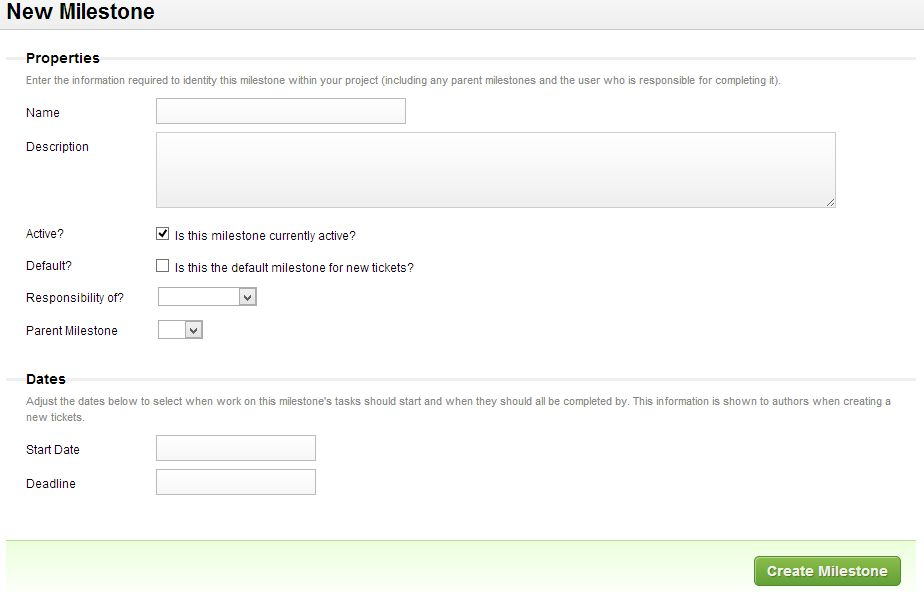
\includegraphics[width=\textwidth]{creazione_milestone}
\caption{Creazione di una nuova Milestone} \label{fig:creazione_milestone}
\end{figure}
Il \underline{form} va completato nel seguente modo:
\begin{itemize}
\item \textbf{Name}: inserire il nome della \underline{Milestone};
\item \textbf{Description}: inserire una breve descrizione della \underline{Milestone};
\item \textbf{Active?}: \underline{flag} da spuntare se si vuole che la \underline{Milestone} creata sia quella attiva;
\item \textbf{Default?}: \underline{flag} da spuntare se si vuole che i futuri \underline{tickets} creati siano riferiti a questa \underline{Milestone};
\item \textbf{Responsibility of?}: selezionare la persona responsabile;
\item \textbf{Parent \underline{Milestone}}: selezionare se la \underline{Milestone} che si va a creare è figlia di qualche altra \underline{Milestone};
\item \textbf{Start Date}: inserire la data da cui far iniziare la \underline{Milestone};
\item \textbf{Deadline}: inserire la data di chiusura delle \underline{Milestone}.
\end{itemize}
Nel caso non si conosca qualche informazione, si può lasciare il relativo campo bianco e modificarlo successivamente (vedi paragrafo seguente) quando sarà resa pubblica l'informazione.

\subsubsection{Modifica Milestone}
Per modificare una \underline{Milestone}, ci si deve posizionare nella scheda ``Edit \underline{Milestone}''. Per raggiungerla, basta entrare nella \underline{Milestone} che si vuole modificare e cliccare sul bottone ``Edit \underline{Milestone}'' situato nella parte alta dello schermo a destra.
\begin{figure}[h]
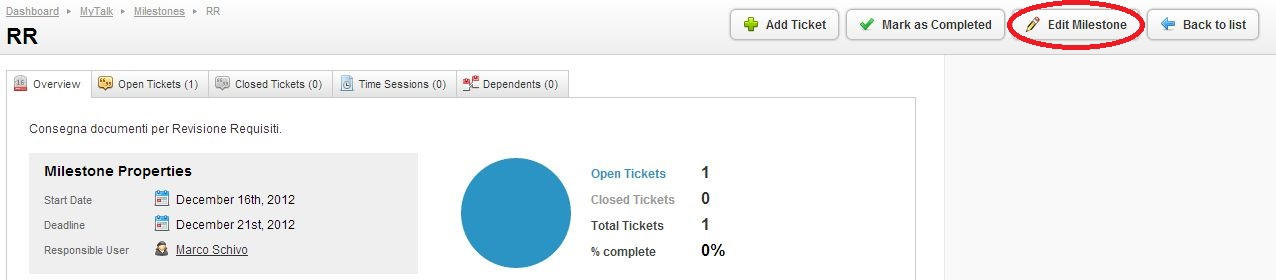
\includegraphics[width=\textwidth]{modifica_milestone}
\caption{Modifica di una Milestone} \label{fig:modifica_milestone}
\end{figure}
\\Per la compilazione dei campi, valgono le stesse regole riportate nella sezione \ref{sec:creazione_milestone} ``Creazione nuova \underline{Milestone}''.
\\Da notare che si può eliminare anche una \underline{Milestone} da tale scheda, basta cliccare sul bottone ``Delete Milestone'' presente nella parte destra della pagina.

\subsection{Ticketing}
Un \underline{ticket} rappresenta un compito da svolgere.

\subsubsection{Creazione nuovo Ticket}
\label{sec:creazione_ticket}
Per inserire un nuovo \underline{ticket} ci si dovrà posizionare nella pagina web dedicata ai \underline{Tickets} e cliccare su ``New Ticket''.
\begin{figure}[h]
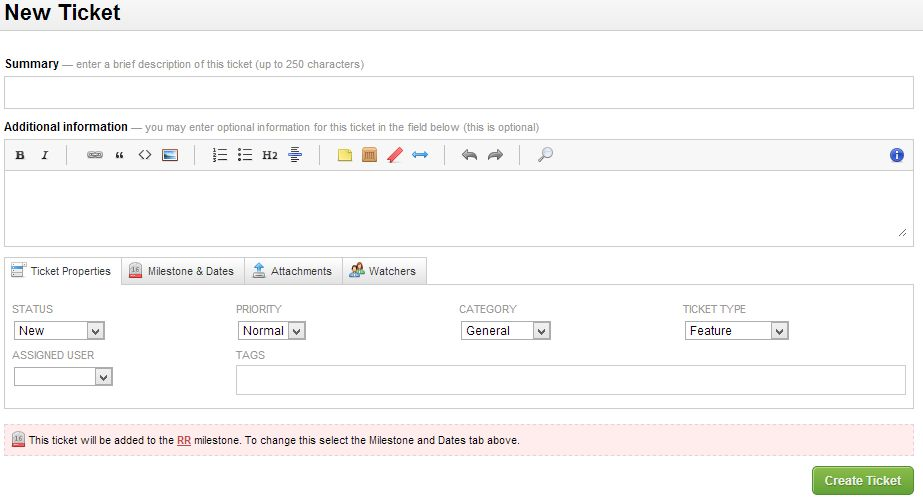
\includegraphics[width=\textwidth]{creazione_ticket}
\caption{Creazione di un nuovo Ticket} \label{fig:creazione_ticket}
\end{figure}
Il \underline{form} va completato compilando obbligatoriamente i seguenti campi:
\begin{itemize}
\item \textbf{Summary}: inserire il nome del compito da assegnare;
\item \textbf{Status}: da settare su ``New'';
\item \textbf{Priority}: selezionare la priorità effettiva del compito;
\item \textbf{Ticket Type}: da settare su ``Task'';
\item \textbf{Assigned User}: selezionare la persona che dovrà svolgere il compito;
\item \textbf{\underline{Milestone}}: selezionare la \underline{Milestone} corrispondente del compito.
\end{itemize}
Tutte le altre informazioni possono essere completate se si ritiene opportuno dare maggiori dettagli.

\subsubsection{Modifica Ticket}
Durante l'intero ciclo di vita di un \underline{ticket}, questo viene modificato molte volte come avviene ad esempio quando dobbiamo modificare lo stato del \underline{ticket}. Per far ciò, basta entrare nel \underline{ticket} che si vuole modificare e appare subito la scheda di modifica.
\begin{figure}[h]
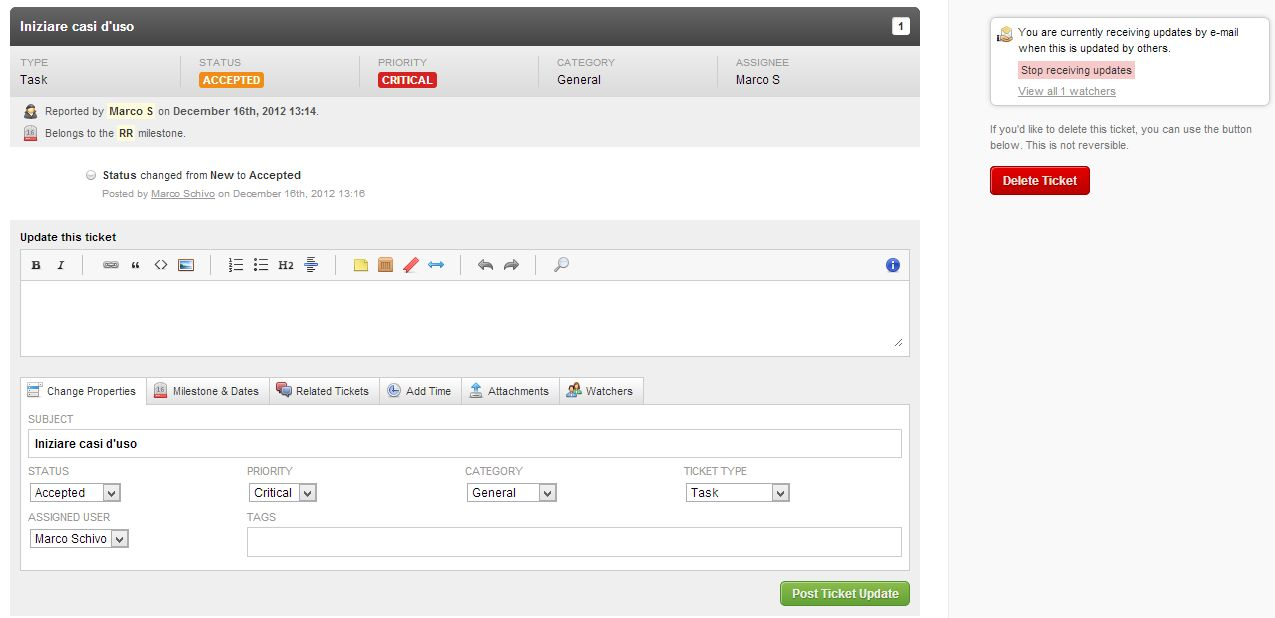
\includegraphics[width=\textwidth]{modifica_ticket}
\caption{Modifica di un ticket} \label{fig:modifica_ticket}
\end{figure}

\subsubsection{Ciclo di vita di un Ticket}
\label{sec:ciclo_vita_ticket}
\begin{enumerate}
\item \textbf{Creazione}: come prima cosa, il \underline{ticket} va creato come descritto nella sezione \ref{sec:creazione_ticket} ``Creazione nuovo Ticket''.
\item \textbf{Esecuzione}: ogni membro dovrà prendere atto dei \underline{tickets} a lui pervenuti e una volta visionati impostare lo stato ad ``Accepted'' o ad ``Invalid''. Una volta accettati, lo stato va modificato in ``In Progress'' quando si inizia a lavorarci e ``Completed'' quando si è portato a termine il compito assegnato.
\item \textbf{Verifica}: una volta che il compito è stato completato, si procede nella creazione di un nuovo \underline{ticket} di tipo ``Verification'' il quale verrà assegnato ad un verificatore. Il nuovo \underline{ticket} va compilato nel seguente modo:
\begin{itemize}
\item \textbf{Summary}: dovrà contenere il nome del documento o file da verificare;
\item \textbf{Status}: da settare su ``New'';
\item \textbf{Priority}: selezionare la priorità effettiva del compito;
\item \textbf{Ticket Type}: da settare su ``Verification'';
\item \textbf{Assigned User}: selezionare il verificatore che dovrà svolgere il compito;
\item \textbf{Milestone}: selezionare la \underline{Milestone} entro cui il documento dovrà essere verificato.
\end{itemize}
\item \textbf{Esecuzione verifica}: per ogni errore (esclusi quelli grammaticali) dovrà essere creato un nuovo \underline{ticket} nel seguente modo:
\begin{itemize}
\item \textbf{Summary}: dovrà contenere il nome del documento o file da modificare;
\item \textbf{Additional information}: dovrà contenere la descrizione dell'errore presente nel documento;
\item \textbf{Status}: da settare su ``New'';
\item \textbf{Priority}: selezionare la priorità effettiva del compito;
\item \textbf{Ticket Type}: da settare su ``Bug'';
\item \textbf{Assigned User}: selezionare il Responsabile del progetto;
\item \textbf{Milestone}: selezionare la \underline{Milestone} entro cui il documento dovrà essere verificato.
\end{itemize}
Sarà  compito del Responsabile approvare o invalidare il \underline{ticket}. In caso di approvazione, il Responsabile dovrà decidere a chi far eseguire la modifica. Il membro selezionato dovrà quindi risolvere l'errore. Una volta completata la modifica il Responsabile dovrà riapplicare la procedura a partire dal punto 3.
\end{enumerate}
Quando tutti i \underline{tickets} di una \underline{Milestone} avranno stato ``Completed'', significa che tutte le attività sono state svolte e il Responsabile potrà procedere alla chiusura della \underline{Milestone}.

\newpage
\section{Analisi dei Requisiti}
L'analisi dei requisiti dovrà essere redatta dagli analisti. Il documento si presenterà suddiviso principalmente in tre parti: una prima parte riguardante i requisiti, una seconda parte riguardante i casi d'uso e la parte finale riguardante il tracciamento dei due elementi appena elencati.

\subsection{Norme per i requisiti}
La parte riguardante i requisiti dovrà elencare ordinatamente tutti i requisiti evinti dal capitolato d'appalto o dagli incontri con il proponente. Per far ciò, \textit{ogni requisito avrà nome univoco} e dovrà essere indicato nel formalismo:
\begin{center}
R\{Ambito\}\{Tipo\}\{Priorità\}\{Gerarchia\}
\end{center}
dove:
\begin{itemize}
\item \textbf{Ambito}: indicherà l'ambito del requisito e potrà assumere i seguenti valori
\begin{itemize}
\item U per indicare ``Utente'';
\item S per indicare ``di Sistema''.
\end{itemize}
\item \textbf{Tipo}: indicherà il tipo del requisito e potrà assumere i seguenti valori:
\begin{itemize}
\item F per indicare ``Funzionale'', ossia requisiti che definiscono quali funzioni devono essere comprese. Tali requisiti si verificano per mezzo di test, dimostrazioni formali e revisioni.
\item Q per indicare ``di Qualità'', ossia definisce i requisiti sui fattori di rilievo della qualità, usabilità, sicurezza, scalabilità. Per questi deve essere adoperata una verifica ad hoc.
\item P per indicare ``Prestazionale'', ossia requisiti che stabiliscono vincoli su tempistiche e spazio, in relazione alla funzione da svolgere. Vengono verificati tramite misurazioni.
\item D per indicare ``Dichiarativo'', ossia requisiti con vincoli spesso ambientali e culturali. Si verificano per mezzo di revisione.

\end{itemize}
\item \textbf{Priorità}: indicherà la priorità del requisito e potrà assumere i seguenti valori
\begin{itemize}
\item O per indicare ``Obbligatorio'', ossia necessario per la realizzazione del progetto;
\item D per indicare ``Desiderabile'', ossia non obbligatorio ma, se implementato, aumenta il valore del progetto;
\item F per indicare ``Facoltativo'', ossia un requisito da implementare se avanzano risorse al termine del progetto.
\end{itemize}
\item \textbf{Gerarchia}: indicherà il grado di parentela dei requisiti e andrà specificato nella sintassi
\begin{center}
\textit{x.y.z}
\end{center}
dove il numero più a sinistra rappresenta il padre e quelli più a destra i figli.
\end{itemize}
Ogni requisito dovrà essere presente nel documento attraverso una ``scheda'', dove oltre i dettagli ricavabili dal nome, dovranno essere specificati anche una breve descrizione, la fonte (ossia la loro origine) e il motivo.\\\\
\textit{Esempio}\\
``RUFO2.3.1'' indica un requisito utente, funzionale obbligatorio con padre RUFO2.3.0 che a sua volta è figlio di RUFO2.0.0.

\subsection{Norme per i casi d'uso}
Il nome di ogni caso d'uso dovrà essere anch'esso, come per i requisiti, univoco e nella forma:
\begin{center}
UC\{n1.n2...n3\}
\end{center}
dove con ``{n1.n2...n3\}'' intendiamo la gerarchia, ossia il grado di parentela. Come per i requisiti, il numero più a sinistra rappresenta il padre e quelli più a destra i suoi figli.\\
Ogni caso d'uso dovrà avere i seguenti dettagli:
\begin{itemize}
\item Nome;
\item Grafico UML;
\item Scopo;
\item Pre;
\item Post;
\item Attori;
\item Scenario Principale;
\item Scenari Secondari.    
\end{itemize}
\textit{Esempio}\\
``UC1.2.3.0'' indica un caso d'uso con padre UC1.2.0 che a sua volta è figlio di UC1.0.0.

\subsection{Tracciamento}
Durante l'intero ciclo di vita del progetto, sono previste misure per il tracciamento dei casi d'uso con i relativi requisiti. Questo avviene grazie all'utilizzo del sistema di tracciamento dei requisiti ``\manager{}'' descritto nella sezione \ref{sec:tracciamento} ``Sistema di tracciamento dei requisiti''. Tutta la gestione è automatica e in output sarà visualizzata una tabella con tre colonne: Codice UC, Nome UC, Requisito. Questa soluzione facilita notevolmente la gestione di grandi quantità di dati e un notevole risparmio di tempo.

\newpage
\section{Norme di verifica}
La verifica è un'attività molto importante svolta dal verificatore. Lo scopo è di accertare che i prodotti ottenuti, qualunque sia il loro tipo, siano conformi le norme e convenzioni riportate su questo documento. Oltre a questo, il verificatore dovrà anche assicurare sotto la propria responsabilità che tali prodotti rispettino i requisiti di qualità descritti nel documento Piano di Qualifica (piano\_di\_qualifica.1.0.pdf).

\subsection{Verifica dei documenti}
\label{sec:verifica_documenti}
La verifica di un documento avviene nel momento in cui il redattore ha finito di redigere completamente il documento. Tale processo avverrà principalmente in tre fasi:
\begin{enumerate}
\item Si procederà con un'analisi ortografica, compreso il corretto uso della punteggiatura, degli accenti e degli apostrofi. Per far ciò il verificatore potrà aiutarsi con lo strumento ``Verifica ortografia'' presente in TexMaker raggiungibile dalla scheda ``Modifica->Verifica Ortografia''. Successivamente controllerà l'assenza di errori grammaticali, logici e sintattici nei periodi ed infine la coerenza del documento con le norme previste nella sezione \ref{sec:ambiente_documentale} ``Ambiente documentale''.
\item Se è la prima volta che il documento viene verificato, il verificatore procederà con un metodo di tipo \underline{walkthrougth}, ossia analizzerà l'intero documento dall'inizio alla fine. Se invece il documento era già stato verificato e rimandato per via di errori, si adopererà un metodo di tipo \underline{inspection}, ossia analizzerà il documento solo dove sono state apportate le modifiche accertandosi che siano stati corretti gli errori rilevati e che non ne siano stati introdotti nuovi.
\item Il verificatore prenderà nota in modo ordinato di tutti gli errori riscontrati e procederà con la creazione dei \underline{tickets} relativi che saranno rivolti al redattore del documento come descritto nella sezione \ref{sec:ciclo_vita_ticket} ``Ciclo di vita di un \underline{Ticket}''.
\end{enumerate}

\end{document}